\documentclass[12pt,border=1pt]{standalone}
\usepackage[T1]{fontenc}
\IfFileExists{newtxtext.sty}{\usepackage{newtxtext,newtxmath}}{\usepackage{mathptmx}}
\usepackage{amsmath,amssymb}
\usepackage[table]{xcolor}
\usepackage{tikz}
\usetikzlibrary{arrows.meta,positioning,fit,calc,decorations.pathreplacing}
\tikzset{blk/.style={draw=black!55,rounded corners=2pt,align=center,font=\footnotesize,inner sep=4pt,minimum height=1.05cm},
         nn/.style={blk,fill=orange!12,draw=orange!70!black},
         lat/.style={blk,fill=blue!8,draw=blue!60!black},
         io/.style={blk,fill=black!3},
         arr/.style={-{Stealth[length=2.2mm]},thick,draw=black!65}}
\definecolor{capblue}{RGB}{47,84,150}
\definecolor{linkblue}{RGB}{17,85,204}
\definecolor{ganttA}{RGB}{11,90,110}
\definecolor{ganttB}{RGB}{20,150,160}
\definecolor{rowhl}{RGB}{253,236,224}
\definecolor{rowhl2}{RGB}{224,244,238}
\begin{document}
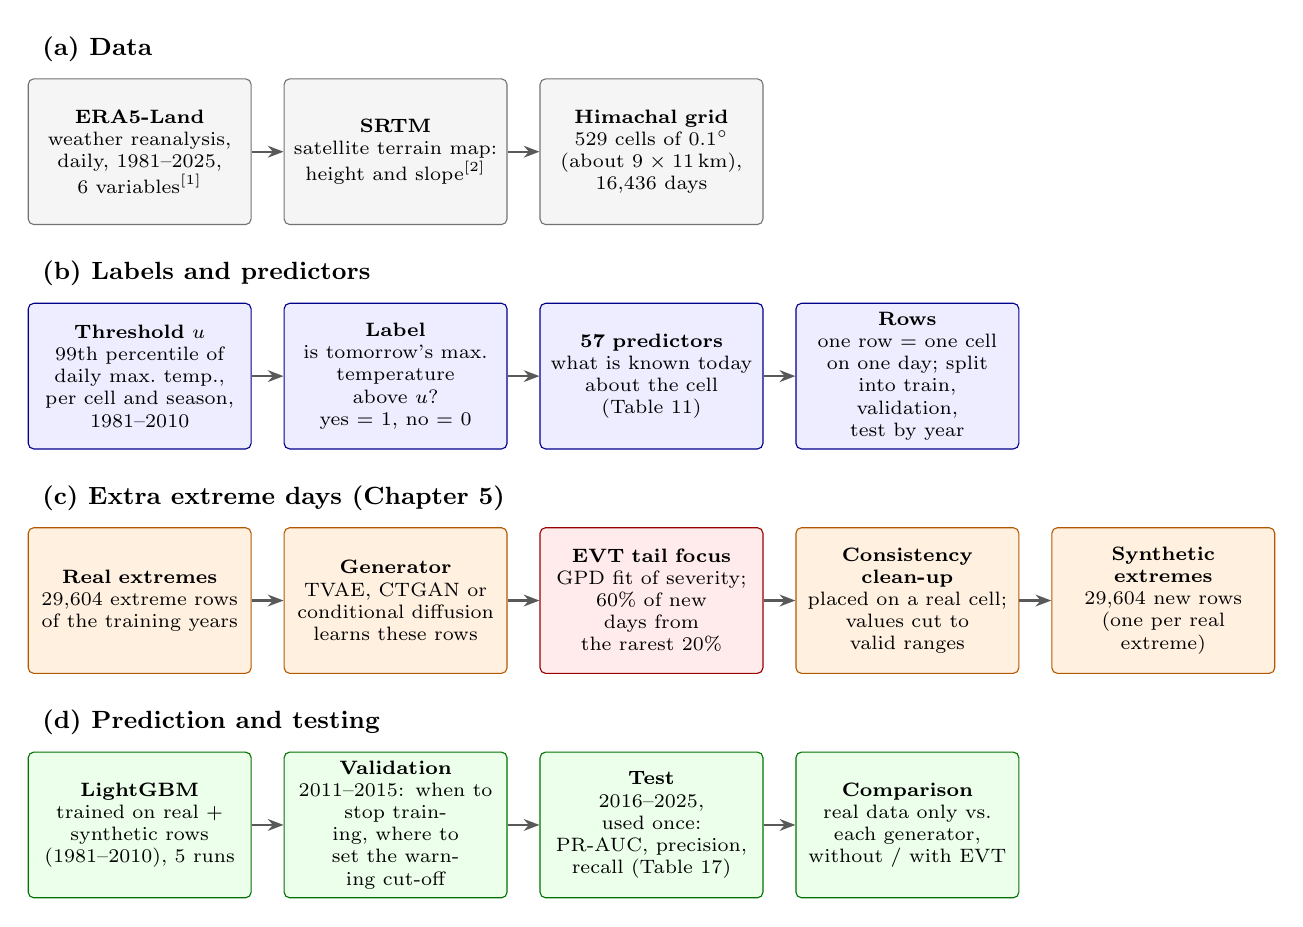
\begin{tikzpicture}[
  st/.style={draw=black!55,rounded corners=2pt,align=center,font=\scriptsize,text width=2.62cm,minimum height=1.85cm,inner sep=3pt},
  dat/.style={st,fill=black!4},
  lab/.style={st,fill=blue!7,draw=blue!55!black},
  gen/.style={st,fill=orange!12,draw=orange!70!black},
  evt/.style={st,fill=red!8,draw=red!60!black},
  clf/.style={st,fill=green!8,draw=green!45!black},
  hd/.style={font=\small\bfseries,anchor=west},
  ar/.style={-{Stealth[length=2mm]},thick,draw=black!65}]
% (a) data
\node[hd] at (-1.36,1.3) {(a) Data};
\node[dat] (a1) at (0,0) {\textbf{ERA5-Land}\\weather reanalysis,\\daily, 1981--2025,\\6 variables$^{[1]}$};
\node[dat] (a2) at (3.25,0) {\textbf{SRTM}\\satellite terrain map:\\height and slope$^{[2]}$};
\node[dat] (a3) at (6.5,0) {\textbf{Himachal grid}\\529 cells of 0.1$^\circ$\\(about $9\times11$\,km),\\16{,}436 days};
\draw[ar] (a1) -- (a2); \draw[ar] (a2) -- (a3);
% (b) labels and predictors
\node[hd] at (-1.36,-1.55) {(b) Labels and predictors};
\node[lab] (b1) at (0,-2.85) {\textbf{Threshold $u$}\\99th percentile of\\daily max.\ temp.,\\per cell and season,\\1981--2010};
\node[lab] (b2) at (3.25,-2.85) {\textbf{Label}\\is tomorrow's max.\\temperature above $u$?\\yes = 1, no = 0};
\node[lab] (b3) at (6.5,-2.85) {\textbf{57 predictors}\\what is known today\\about the cell\\(Table~11)};
\node[lab] (b4) at (9.75,-2.85) {\textbf{Rows}\\one row = one cell\\on one day; split\\into train, validation,\\test by year};
\draw[ar] (b1) -- (b2); \draw[ar] (b2) -- (b3); \draw[ar] (b3) -- (b4);
% (c) extra extremes
\node[hd] at (-1.36,-4.4) {(c) Extra extreme days (Chapter~5)};
\node[gen] (c1) at (0,-5.7) {\textbf{Real extremes}\\29{,}604 extreme rows\\of the training years};
\node[gen] (c2) at (3.25,-5.7) {\textbf{Generator}\\TVAE, CTGAN or\\conditional diffusion\\learns these rows};
\node[evt] (c3) at (6.5,-5.7) {\textbf{EVT tail focus}\\GPD fit of severity;\\60\% of new days from\\the rarest 20\%};
\node[gen] (c4) at (9.75,-5.7) {\textbf{Consistency clean-up}\\placed on a real cell;\\values cut to\\valid ranges};
\node[gen] (c5) at (13.0,-5.7) {\textbf{Synthetic extremes}\\29{,}604 new rows\\(one per real\\extreme)};
\draw[ar] (c1) -- (c2); \draw[ar] (c2) -- (c3); \draw[ar] (c3) -- (c4); \draw[ar] (c4) -- (c5);
% (d) prediction and testing
\node[hd] at (-1.36,-7.25) {(d) Prediction and testing};
\node[clf] (d1) at (0,-8.55) {\textbf{LightGBM}\\trained on real +\\synthetic rows\\(1981--2010), 5 runs};
\node[clf] (d2) at (3.25,-8.55) {\textbf{Validation}\\2011--2015: when to\\stop training, where to\\set the warning cut-off};
\node[clf] (d3) at (6.5,-8.55) {\textbf{Test}\\2016--2025, used once:\\PR-AUC, precision,\\recall (Table~17)};
\node[clf] (d4) at (9.75,-8.55) {\textbf{Comparison}\\real data only vs.\\each generator,\\without / with EVT};
\draw[ar] (d1) -- (d2); \draw[ar] (d2) -- (d3); \draw[ar] (d3) -- (d4);
\end{tikzpicture}
\end{document}
